\chapter{Analyse et solution du problème}
\chaptermark{Analyse du P}

\section{Introduction et choix du langage}
Dans le cadre du module Systèmes Distribués, l'opportunité de  spécifier et concevoir  un générateur de tâches temps réel nous est proposé. Le langage d'implémentation étant libre, notre binome a opté pour Java. Ce choix est basé principalement par le fait qu'il s'agissait du langage le mieux maitrisé. Cela nous a permis de concentrer nos efforts sur la mise en place des algorithmes et non sur des probèmes de langage.
 L'objectif est de définir un outil de simulation  d'ordonnancement de tâches en temps réel.

\section{Modelisation du problème}
Suite à l'étude du cahier des charges nous proposons l'architecture de l'outil suivante :
   \begin{figure}[htbp]
  \centering
  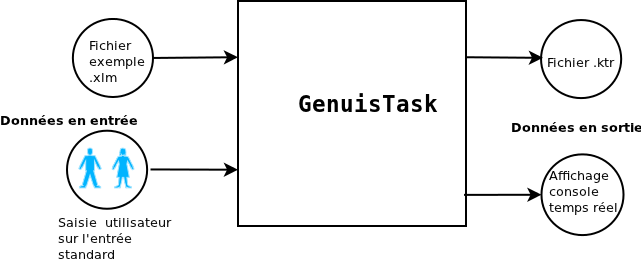
\includegraphics[scale=0.70]{img/archi}
  \caption{Architecture de l'outil}
  \label{fig:archi}
\end{figure}
\section{Génération de tâches dans un fichier}
\sectionmark{Génération fichier}
La première partie du projet avait pour objectif d'obtenir un nombre $n$ de tâches périodiques et apériodiques pour de futurs traitements décrits dans la seconde partie (\ref{Part2}). \`A nouveau le choix du format d'un tel fichier nous était laissé. Nous avons choisi de générer un fichier xml (à nouveau pour des raisons  de simplicité) à la syntaxe suivante : 

\begin{itemize}
\item
Des balises \verb+<genTache.AbstractTache-array>+ encadrent la totalité du fichier.
\item
Une tâche périodique sera définie dans une balise  \verb+<genTache.TachePeriodique>+ 
\item
Une tâche apériodique sera définie dans une balise  \verb+<genTache.TacheAPeriodique>+ 
\item
Dans une tâche tous ses attributs seront définis de la manière suivante \verb+<nom_attribut>valeur_attribut</nom_attribut>+
\end{itemize}

Voici un exemple d'un fichier respectant le format décrit ci-dessus : 

\begin{lstlisting}
<genTache.AbstractTache-array>
  <genTache.TachePeriodique>
    <Pi>377</Pi>
    <ri>0</ri>
    <id>1</id>
    <Ci>1</Ci>
    <Di>1</Di>
  </genTache.TachePeriodique>
  <genTache.TachePeriodique>
    <Pi>162</Pi>
    <ri>0</ri>
    <id>2</id>
    <Ci>6</Ci>
    <Di>30</Di>
  </genTache.TachePeriodique>
  <genTache.TacheAperiodique>
    <ri>859</ri>
    <id>3</id>
    <Ci>26</Ci>
    <Di>71</Di>
  </genTache.TacheAperiodique>
</genTache.AbstractTache-array>
\end{lstlisting}
On remarque que les taches périodiques sont identifiées par : 
\begin{itemize}
\item
Pi : période d'activation.
\item
ri : date de réveil.
\item
id : L'id de la tâche.
\item
Ci : durée d'exécution maximale.
\item
Di  : délai critique
\end{itemize} 
Alors que les tâches apériodiques ont seulement : 
\begin{itemize}
\item
ri  : date de réveil
\item
id : L'id de la tâche.
\item
Ci : durée d'exécution maximale.
\item
Di : délai critique.
\end{itemize} 


\section{Algorithmes et structures mises en oeuvre}

\sectionmark{Algorithmes}
\subsection{Commentaires sur la première Partie}
   \begin{figure}[htbp]
  \centering
  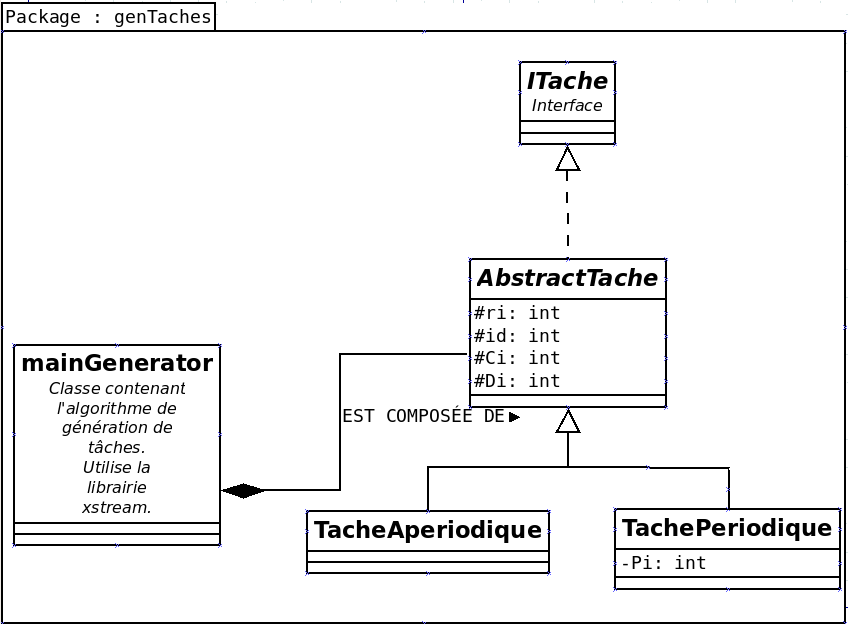
\includegraphics[scale=0.60]{img/packgen}
  \caption{Package générateur de tâches temps réel}
  \label{fig:gen}
\end{figure}

\paragraph{Calcul des tâches apériodiques} 
Le calcul des tâches ap est effectué selon la formule suivante : $ U_a =  \frac{\sum_{i=1}^m C_i}{ppcm(P_i)}$. L'utilisateur entre la variable Uap  et le nombre de tâches apériodiques qu'il désire. 
\paragraph{Détail sur la génération aléatoire}\label{PremPart}
Le cahier des charges spécifiait que la génération se devait d'offrir la possibilité de générer les tâches aléatoirement ou bien en laissant l'utilisateur choisir les paramètres de chacune d'elle. Cependant la génération de tâches aléatoires pose de nombreux problèmes.

Le premier problème est de savoir qu'elle est la taille maximale que l'on peut attribué a un $Ci$ ou un $Pi$. Il aurait été possible de laisser le choix à l'utilisateur mais dès que le nombre de tâches dépasse deux ou que leur $Pi$ est grand, l'hyperpériode explose. L'objectif étant par la suite de pouvoir générer un fichier pour kiwi, il est assez génant d'avoir des durées d'ordonnancements qui dépassent les possibilités des valeurs pour kiwi.

Un autre problème étant de savoir comment générer les tâches pour offrir une palette large vis-à-vis des propriétés des tâches.

Au final le programme de génération des tâches aléatoires est peu sûr et laisse la possibilité, à l'utilisateur, d'entrer des informations contradictoires qui peuvent, dans la majorité des cas, faire échouer la génération.
Par exemple l'utilisateur peut rentrer un nombre de tâches apériodiques non nulle mais mettre ensuite une utilisation processeur nulle pour ces mêmes tâches, ayant pour conséquence de retourner une erreur lors de la génération.

\subsection{Deuxième partie}\label{Part2}
La deuxième partie du projet, consistait à partir du fichier de tâches (cf Première Partie), de créer un simulateur proposant  deux types de fonctionnalités :
\begin{itemize}
\item
une analyse d'ordonnançabilité,
\item
un environnement de simulation.
\end{itemize}
Le premier sujet de réflexion était de savoir dans quelles structures de données stocker les tâches et par quels moyens. Le choix des ArrayList s'est fait naturellement grâce en premier lieu à sa facilité de manipulation. Par ailleurs la fonctionnalité de la bibliothèque xtream permettant d'extraire le contenu d'un fichier xml dans une ArrayList en quelques lignes nous a d'emblée convaincue. Une fois cette première difficulté franchie une seconde de taille est apparue. Nous avons compris qu'il serait délicat de modifier directement les tâches dans les ArrayList. Notre idée initiale était de  modifier le Ci d'une  tâche après son traitement dans l'algorithme. Ce qui dans le cas des tâches périodiques par exemple, serait problématique. En effet par définition les taches périodiques  sont susceptibles  d'être traitées à plusieurs reprises. Il faut donc garder leurs propiétés initiales intactes. Nous avons donc choisi d'organiser notre programmation en plusieurs classes pour bien séparer les opérations de manipulation des données d'une part, les opérations mettant en jeux les algorithmes d'ordonancement et enfin celles écrivant dans le fichier de sortie au format .ktr

   \begin{figure}[htbp]
  \centering
  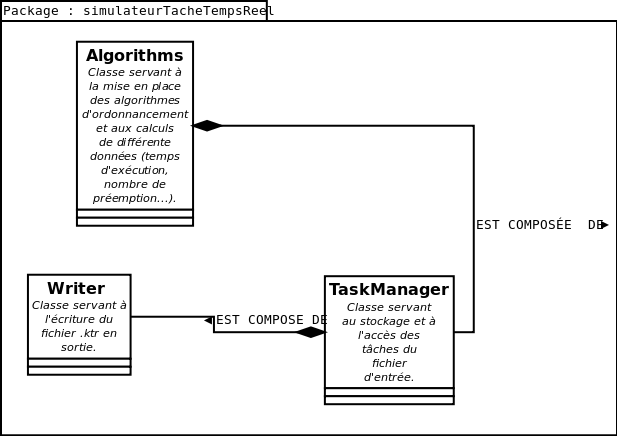
\includegraphics[scale=0.55]{img/packsstr}
  \caption{Package : Simulateur de systèmes temps réel}
  \label{fig:sstr}
\end{figure}
%\clearpage
\section{Interface proposée}
Toutes l'interface de l'outil est en ligne de commande. L'absence d'IHM graphique est due au manque de temps et au peu d'intêret que cela représentait pour le problème étudié. De même l'outil ne prend en compte aucune option. Même si cet aspect aurait apporté un certain confort à l'utilisateur, nous avons opté pour la solution de lui demandé au fur et à mesure de l'exécution du programme les diverses options et paramètres requis. Nous avons regretté ce choix lors de la phase des tests (la répétition sans cesse des divers options est fastidieuse). Cependant nous avons gagné un temps de conception non négligeable. 


